\documentclass[12pt,a4paper]{article}
\usepackage{ctex}
\usepackage{amsmath,amscd,amsbsy,amssymb,latexsym,url,bm,amsthm}
\usepackage{epsfig,graphicx,subfigure}
\usepackage{enumitem,balance}
\usepackage{wrapfig}
\usepackage{mathrsfs,euscript}
\usepackage[usenames]{xcolor}
\usepackage{hyperref}
\usepackage[vlined,ruled,linesnumbered]{algorithm2e}
\usepackage{array}
\hypersetup{colorlinks=true,linkcolor=black}

\usepackage{attachfile}
\usepackage{listings}
\usepackage{amsmath}
\usepackage{booktabs}
\usepackage{threeparttable}
\usepackage{graphicx} %插入图片的宏包
\usepackage{float} %设置图片浮动位置的宏包
\usepackage{subfigure} %插入多图时用子图显示的宏包
\usepackage{natbib}
\usepackage{amssymb,amsmath}
\usepackage{color}
\usepackage{multirow}

\newtheorem{theorem}{Theorem}
\newtheorem{lemma}[theorem]{Lemma}
\newtheorem{proposition}[theorem]{Proposition}
\newtheorem{corollary}[theorem]{Corollary}
\newtheorem{exercise}{Exercise}
\newtheorem*{solution}{Solution}
\newtheorem{definition}{Definition}
\theoremstyle{definition}

\renewcommand{\thefootnote}{\fnsymbol{footnote}}

\newcommand{\postscript}[2]
 {\setlength{\epsfxsize}{#2\hsize}
  \centerline{\epsfbox{#1}}}

\renewcommand{\baselinestretch}{1.0}

\setlength{\oddsidemargin}{-0.365in}
\setlength{\evensidemargin}{-0.365in}
\setlength{\topmargin}{-0.3in}
\setlength{\headheight}{0in}
\setlength{\headsep}{0in}
\setlength{\textheight}{10.1in}
\setlength{\textwidth}{7in}
\makeatletter \renewenvironment{proof}[1][Proof] {\par\pushQED{\qed}\normalfont\topsep6\p@\@plus6\p@\relax\trivlist\item[\hskip\labelsep\bfseries#1\@addpunct{.}]\ignorespaces}{\popQED\endtrivlist\@endpefalse} \makeatother
\makeatletter
\renewenvironment{solution}[1][Solution] {\par\pushQED{\qed}\normalfont\topsep6\p@\@plus6\p@\relax\trivlist\item[\hskip\labelsep\bfseries#1\@addpunct{.}]\ignorespaces}{\popQED\endtrivlist\@endpefalse} \makeatother

\begin{document}
\noindent

%========================================================================
\noindent\framebox[\linewidth]{\shortstack[c]{
\Large{\textbf{Lab08-Graph Exploration}}\vspace{1mm}\\
CS214-Algorithm and Complexity, Xiaofeng Gao \& Lei Wang, Spring 2021.}}
\begin{center}
\footnotesize{\color{red}$*$ If there is any problem, please contact TA Yihao Xie. }

\footnotesize{\color{blue}$*$ Name:Zirui Liu  \quad Student ID: 519021910343 \quad Email: L.prime@sjtu.edu.cn}
\end{center}

\begin{enumerate}

	\item Given an undirected graph $G = (V, E)$. Prove the following propositions.
	
	\begin{enumerate}
		\item Let $e$ be a maximum-weight edge on some cycle of connected graph $G=(V,E)$.
        Then there is a minimum spanning tree of $G$ that does not include $e$. Moreover, there is no minimum spanning tree of $G$ that includes $e$ if $e$ is the unique maximum-weight edge on the cycle. 
		\item Let $T$ and $T'$ are two different minimum spanning trees of $G$. Then $T'$ can be obtained from $T$ by repeatly substitute one edge in $T\backslash T'$ by one edge in $T'\backslash T$ and meanwhile the result after each subsitution is still a minimum spanning tree.
	\end{enumerate}
	
	\begin{solution}
	
	(a):\\
	We suppose that $T$ is a spanning tree of minimum weight, and
    there exists a cycle $C$ so that $e$ is the heaviest edge in $C$ and $e \in E\left(T\right)$. Let $e$ connects two points $u$, $v$
    and let $P = C − e$, so that $p$ is also a path from $u$ to $v$. Now $T − e$ are consists of two parts, as $T_1$ and $T_2$
    while one contains $u$ and the other one contains $v$. Since $P$ is a path from $u$ to $v$, there exists an edge $f \in E\left(P\right) $ with one end in $T_1$ and the other one in $T_2$. By assumption we have
    $w\left(f\right) < w\left(e\right)$, now $T − e + f$ is a spanning tree with weight less than $T$, which made a contradiction. So the original problem can be solved. For the next question, if $e$ is the unique maximum-weight edge on the cycle, there would always be another path having less weight that can replace $e$, so in contradiction, there is no minimum spanning tree of $G$ that includes $e$ if $e$ is the unique maximum-weight edge on the cycle.
	
	
	(b):\\
	We approve by contradiction. If this is not true, assume after one replacement, we got a new $T_i$ that is not a minimum spanning tree, assume that we just use $x_i$ to replace $x$, then we can use $x_i$ to replace $x$ at first, for original $T$, so we can get a better structure for $T$. The $T$ we modified uses less weight to connect all points, lesser then $T$. So $T$ is not a minimum spanning tree, contradiction. In conclusion, the result after each subsitution is still a minimum spanning tree.
	
	
	\end{solution}
	
	
    \item Let $G=(V,E)$ be a connected, undirected graph. Give an $O(|V|+|E|)$-time algorithm
    to compute a path in $G$ that traverses each edge in $E$ exactly once in each direction. Describe how you can find your way out of a maze if you are given enough coins to apply your algorighm.

    \begin{solution}
    1. We first perform a DFS for $G$, starting at an arbitrary vertex.( The path required by the problem can be obtained in the order which DFS 
    explores in the graph.) \\
    2. When exploring an edge $\left(u, v\right)$ that goes to an unvisited vertex, the edge $\left(u, v\right)$ is included for the first time in the path. \\
    3. When DFS backtracks to $u$ again after $v$ is made BLACK, the edge $\left(u, v\right)$ (which in more precise way is that the edge connecting $u$ and $v$ not considering the direction) is included for the second time in the path, which this time is in the opposite direction. from $v$ to $u$. \\
    4. When DFS explores an edge $\left(u, v\right)$ that goes to a pre-visited node (GRAY or BLACK), we add $\left(u, v\right)$ and $\left(v, u\right)$ to the path. In this way we can make sure that each edge is added to the path exactly twice. \\
    
    
    \end{solution}
    
    
    
    \item Consider the maze shown in Figure \ref{Fig-Maze}. The black blocks in the figure are blocks that can not be passed through. Suppose the block are explored in the order of right, down, left and up. That is, to go to the next block from $(X,Y)$, we always explore $(X,Y+1)$ first, and then $(X+1,Y)$,$(X,Y-1)$ and$(X-1,Y)$ at last. Answer the following subquestions:
    \begin{enumerate}
        \item Give the sequence of the blocks explored by using DFS to find a path from the "start" to the "finish".
        \item Give the sequence of the blocks explored by using BFS to find the \underline{shortest} path from the "start" to the "finish".
        \item Consider a maze with a larger size. Discuss which of BFS and DFS will be used to find one path and which will be used to find the shortest path from the start block to the finish block.
    \end{enumerate}
    
    \begin{figure}[!htbp]
	\centering
	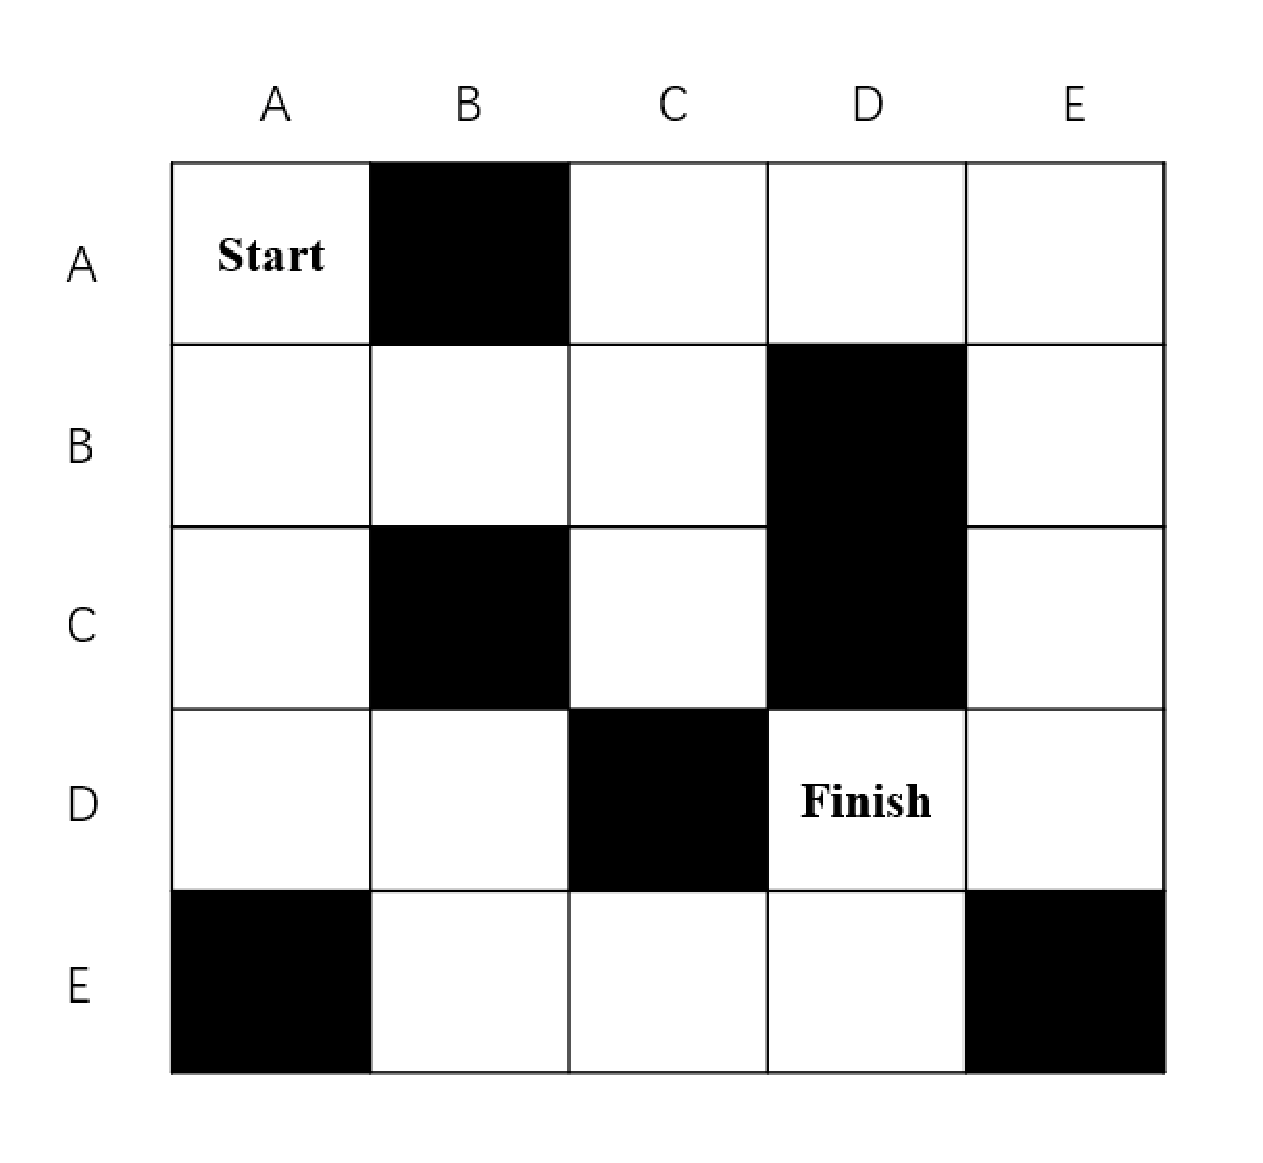
\includegraphics[width=0.45\textwidth]{Fig-Maze.pdf}
	\caption{The blocks in the maze.}
	\label{Fig-Maze}
	\end{figure}
	
	\begin{solution}
	(a):\\
	We give the sequence by $\left(x,y\right)$.
	
	        $\left( A,A \right)$\\
	     -> $\left( B,A \right)$\\
	     -> $\left( B,B \right)$\\
	     -> $\left( B,C \right)$\\
	     -> $\left( C,C \right)$\\
	     -> $\left( B,C \right)$\\
	     -> $\left( A,C \right)$\\
	     -> $\left( A,D \right)$\\
	     -> $\left( A,E \right)$\\
	     -> $\left( B,E \right)$\\
	     -> $\left( C,E \right)$\\
	     -> $\left( D,E \right)$\\
	     -> $\left( D,D \right)$\\
	    
	    
	(b):\\
	\\
	$\left( A,A \right)$\\
	$\left( B,A \right)$\\
	$\left( B,B \right)$\\
	$\left( C,A \right)$\\
	$\left( B,C \right)$\\
	$\left( D,A \right)$\\
	$\left( C,C \right)$\\
	$\left( D,B \right)$\\
	$\left( A,C \right)$\\
	$\left( E,B \right)$\\
	$\left( A,D \right)$\\
	$\left( E,C \right)$\\
	$\left( A,E \right)$\\
	$\left( E,D \right)$\\
	$\left( B,E \right)$\\
	$\left( D,D \right)$\\
	
	(c):\\
	DFS will be used to find one path and BFS will be used to find the shortest path from the start block to the finish block.It's because DFS can get straight to the destination, DFS with backtrack CAN always find a way if there is a way. Otherwise the way does not exist. But DFS can't not get all the different ways od path, so it cannot  know which way is the shortest path. But BFS is different, BFS can get through all the ways possible to get to the end, so BFS can get the shortest way. But if we only need to find if there is a way from  the start to the end, we would only have to apply DFS.
	
	
	\end{solution}
	
	
	\item Given a directed graph $G$, whose vertices and edges information are introduced in data file "SCC.in". Please find its number of Strongly Connected Components with respect to the following subquestions.
    
    \begin{enumerate}
    	\item Read the code and explanations of the provided C/C++ source code "SCC.cpp", and try to complete this implementation.
    	\item Visualize the above selected Strongly Connected Components for this graph $G$. Use the $Gephi$ or other software you preferred to draw the graph. {\color{blue}(If you feel that the data provided in ``SCC.in'' is not beautiful, you can also generate your own data with more vertices and edges than $G$ and draw an additional graph. Notice that results of your visualization will be taken into the consideration of Best Lab.)}
    \end{enumerate}	
\end{enumerate}
    
    \begin{solution}
        \begin{figure}[H] %H为当前位置,!htb为忽略美学标准,htbp为浮动图形
    \centering %图片居中
    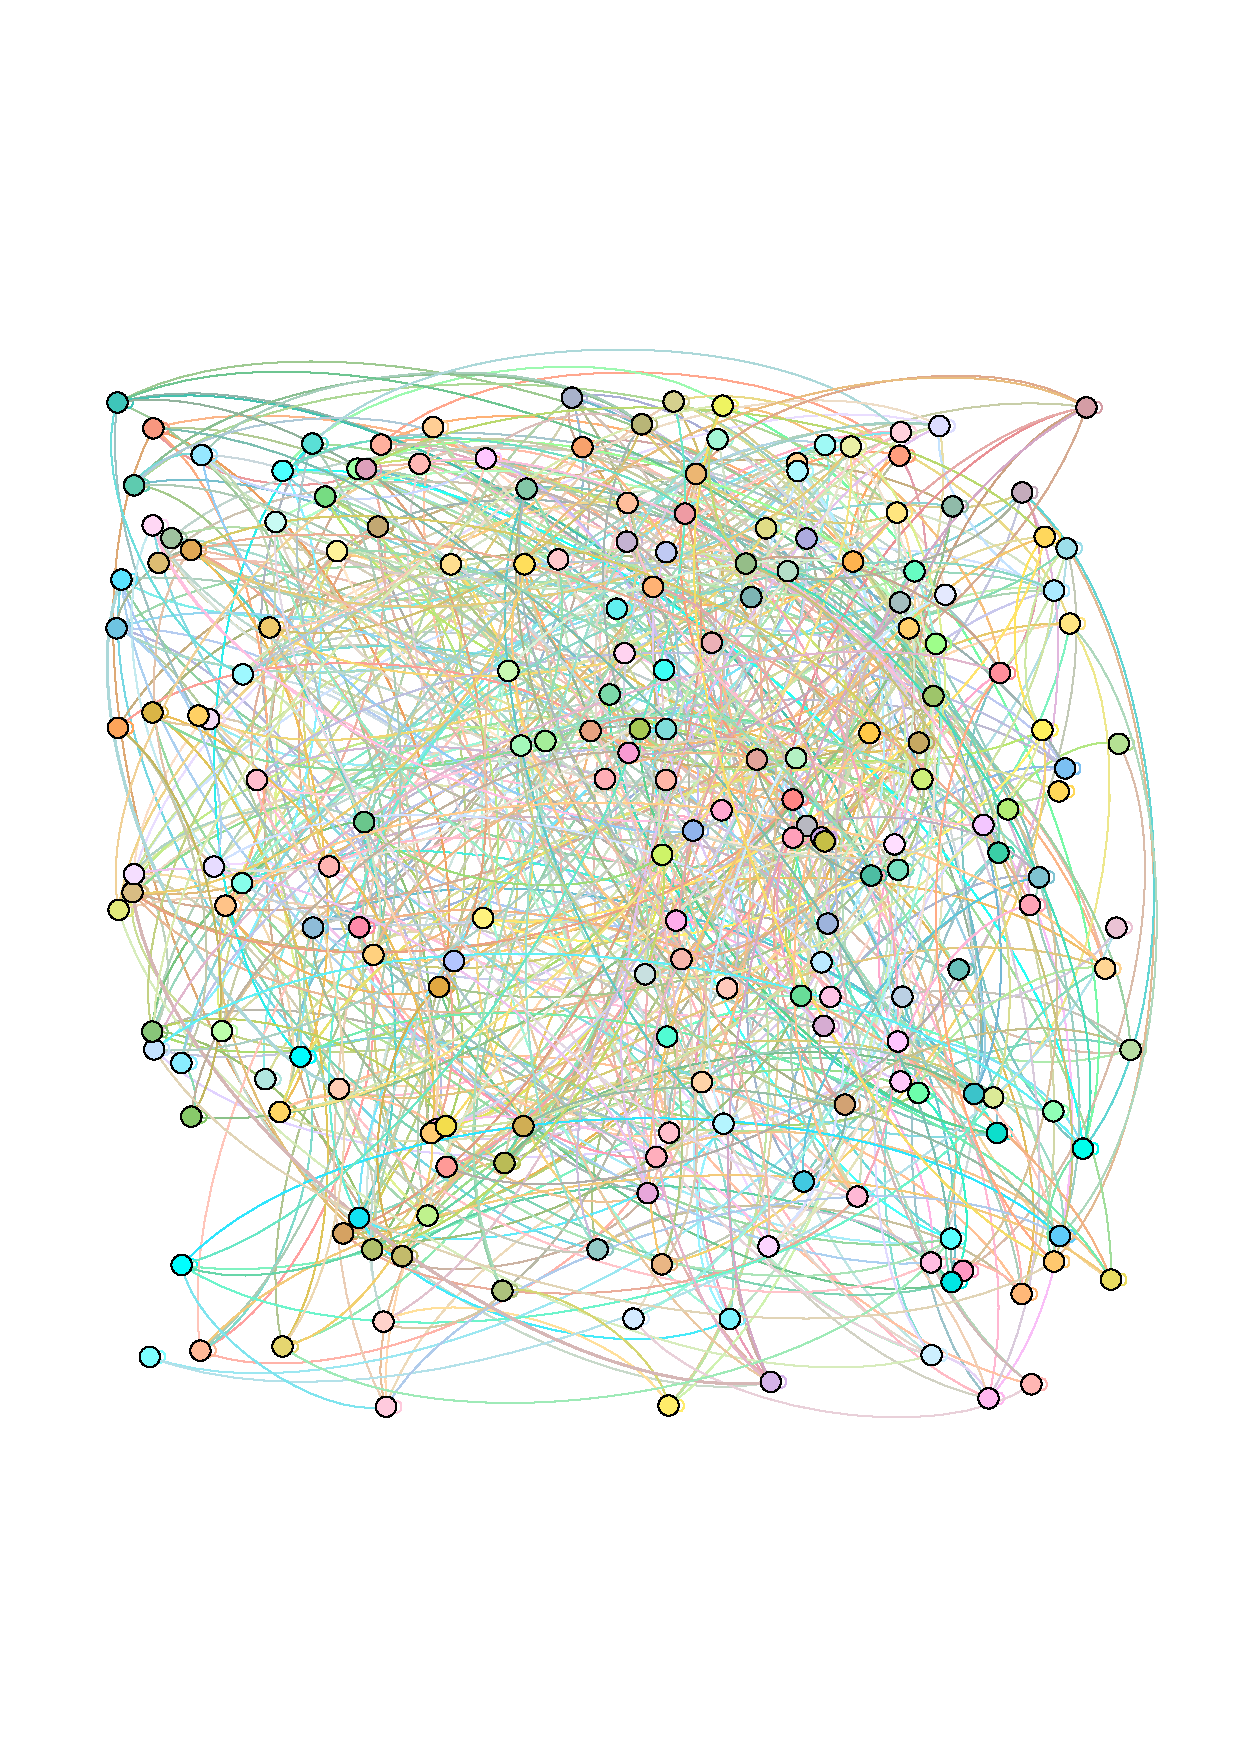
\includegraphics[width=0.5\textwidth]{gephi.pdf}
     %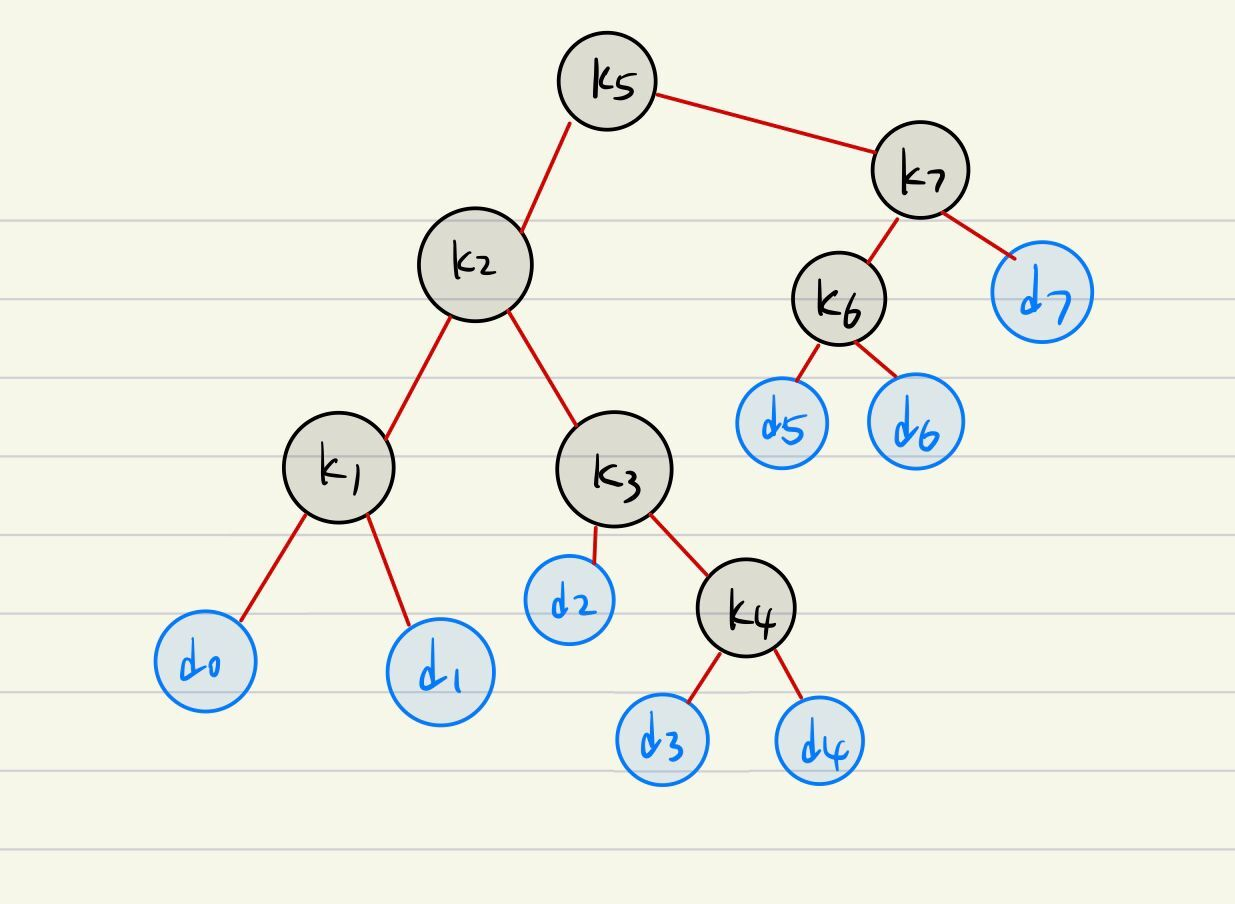
\includegraphics[width=1in]{tree.jpg}
    \caption{picture} %最终文档中希望显示的图片标题
    \label{} %用于文内引用的标签
    \end{figure}
    
    \end{solution}


\textbf{Remark:} Please include your .pdf, .tex, .cpp files for uploading with standard file names.
\newpage


\begin{appendices}
\section{Second appendix: SCC.cpp}
\textcolor[rgb]{0.98,0.00,0.00}{\textbf{Input c++ source1:}}
\lstinputlisting[language=c++]{./SCC.cpp}

\end{appendices}



%========================================================================
\end{document}